\documentclass[UTF8,a4paper,12pt]{ctexart}

\usepackage{geometry}
\usepackage{graphicx}
\usepackage{amsmath}
\usepackage{booktabs}
\usepackage{longtable}
\usepackage{array}
\usepackage{float}
\usepackage{hyperref}
\usepackage{xcolor}
\usepackage{listings}
\usepackage{caption}
\usepackage{subcaption}
\usepackage{enumitem}

\geometry{left=2.5cm,right=2.5cm,top=2.6cm,bottom=2.6cm}
\hypersetup{colorlinks=true,linkcolor=black,urlcolor=blue,citecolor=black}
\setlist[itemize]{leftmargin=2em}
\setlist[enumerate]{leftmargin=2em}
\renewcommand{\arraystretch}{1.25}
\setlength{\emergencystretch}{3em}

\lstset{
  basicstyle=\ttfamily\small,
  breaklines=true,
  frame=single,
  columns=fullflexible,
  keepspaces=true,
  backgroundcolor=\color{gray!6}
}

\title{CSE5023 Assignment 2 实验报告\\\large Transformer 在翻译、情感分析与视觉分类任务中的实现与实验}
\author{姓名：\underline{\hspace{3cm}}\quad 学号：12533582}
\date{\today}

\begin{document}
\maketitle

\begin{abstract}
本文围绕 CSE5023 Assignment 2 的三个任务展开：第一部分实现 English-to-Chinese 机器翻译 Transformer，并完成 baseline、cosine warm-up 学习率调优、结构消融和位置嵌入实验；第二部分复用机器翻译 encoder，在 Tweet Sentiment Extraction 数据集上进行情感分类微调，并比较有无 position encoding 的影响；第三部分在 CIFAR-10 上实现 Vision Transformer，并与 ImageNet 预训练 ResNet50 进行对比。实验结果显示，cosine warm-up 明显提升机器翻译 BLEU，翻译 encoder 对情感分类具有迁移价值，而在 CIFAR-10 小图像分类中，预训练 ResNet50 凭借大规模视觉预训练和 CNN 局部归纳偏置取得了高于从零训练 ViT 的准确率。
\end{abstract}

\tableofcontents
\newpage

\section{第一部分：English-to-Chinese 机器翻译}

本部分按照作业第一章的小节编号逐项展开，覆盖 Transformer 架构实现、baseline 训练与 BLEU 评估、cosine warm-up 学习率调优、结构消融和 position embedding 对比。机器翻译代码位于 \path|code/part1_machine_translation/|，实验结果统一保存到 \path|outputs/part1_machine_translation/|，便于后续情感分析任务加载 encoder checkpoint。

\subsection{1.1 Transformer 架构实现}

本小节对应机器翻译任务的基础架构实现。按照作业要求，本部分主要修改了以下两个代码文件：
\begin{lstlisting}
code/part1_machine_translation/tokenization.py
code/part1_machine_translation/model/transformer.py
\end{lstlisting}

首先修改 \texttt{tokenization.py} 中的 \texttt{wordToID}。原始数据在读取后已经被分成英文 token 序列和中文 token 序列，但模型不能直接处理字符串，因此需要把 token 转换为词表中的整数 id。我在该函数中分别遍历英文句子和中文句子，使用训练集构建出的 \texttt{en\_dict} 和 \texttt{cn\_dict} 完成映射；如果某个词没有出现在词表中，则统一映射为 \texttt{UNK}。转换完成后，再按英文句子长度排序。这样做可以让长度相近的句子更容易被分到相邻 batch 中，减少 padding token 的数量。

然后检查并使用 \texttt{MaskBatch} 完成 batch 级输入组织。Encoder 输入保存在 \texttt{src} 中，\texttt{src\_mask} 通过判断 \texttt{src != pad\_id} 得到，用来屏蔽源句中的 padding 位置。Decoder 端将完整目标句拆成两部分：\texttt{tgt[:, :-1]} 作为 decoder 输入，\texttt{tgt[:, 1:]} 作为预测标签。随后把目标端 padding mask 和 causal mask 组合成 \texttt{tgt\_mask}，保证 decoder 既不会关注 padding，也不会看到未来 token。

接着修改 \texttt{model/transformer.py} 中的 \texttt{FeedForwardBlock}。这一部分对应 Transformer block 里的前馈网络。我实现了两层线性变换，中间加入 ReLU 激活和 dropout，即 \texttt{Linear -> ReLU -> Dropout -> Linear}。前馈网络对序列中的每个位置独立作用，用来增强每个 token hidden state 的非线性表达能力。

之后补全 \texttt{MultiHeadAttentionBlock.attention}。注意力分数先由 query 和 key 的点积得到，并除以 $\sqrt{d_k}$ 进行缩放；如果传入 mask，就在 softmax 之前把被屏蔽的位置填成 $-10^9$，使这些位置在 softmax 后的权重接近 0。最后使用注意力权重对 value 加权求和，返回 attention 输出和 attention scores。这个函数同时服务于 encoder self-attention、decoder masked self-attention 和 decoder cross-attention。

最后确认 \texttt{build\_transformer} 能把各个模块组合成完整模型。模型先建立 source/target embedding 和 sinusoidal position encoding，再堆叠多个 encoder block 和 decoder block，并在 decoder 后接 projection layer，把 hidden state 映射到中文词表空间。这样，整个 English-to-Chinese encoder-decoder Transformer 的前向计算流程就完整连通了。

\subsubsection{整体结构}

本任务实现的是标准 encoder-decoder Transformer。源语言英文句子首先经过 source embedding 与位置编码，然后送入 encoder；目标语言中文序列经过 target embedding 与位置编码后送入 decoder。Decoder 同时接收自身历史输出和 encoder 的输出，最后通过 projection layer 映射到中文词表空间，得到每个位置的词概率分布。

模型中主要组件如下：
\begin{itemize}
  \item \textbf{Embedding}：\texttt{InputEmbeddings} 使用 \texttt{nn.Embedding} 将 token id 映射为 $d_{model}$ 维向量，并乘以 $\sqrt{d_{model}}$，使 embedding 的数值尺度与后续位置编码、注意力计算更匹配。
  \item \textbf{Position Encoding}：\texttt{PositionalEncoding} 使用固定 sinusoidal 位置编码，将序列中每个 token 的位置信息加入 embedding。由于 self-attention 本身不包含顺序信息，位置编码是模型理解词序的必要部分。
  \item \textbf{Multi-Head Attention}：\texttt{MultiHeadAttentionBlock} 将输入投影为 query、key、value，并拆分为多个 head。每个 head 独立计算 scaled dot-product attention，最后拼接并通过输出线性层得到多头注意力结果。
  \item \textbf{Feed Forward Network}：\texttt{FeedForwardBlock} 对每个位置独立执行两层线性变换，中间使用 ReLU 和 dropout，用于增强每个 token 表示的非线性表达能力。
  \item \textbf{Residual Connection 与 LayerNorm}：每个 attention 子层和 FFN 子层外部都使用残差连接与层归一化，帮助深层模型稳定训练并缓解梯度传播困难。
  \item \textbf{Projection Layer}：\texttt{ProjectionLayer} 将 decoder 输出从 $d_{model}$ 维映射到目标词表大小，并使用 log softmax 输出词表概率。
\end{itemize}

\subsubsection{Encoder 与 Decoder 的差异}

Encoder 和 Decoder 都由多层 Transformer block 组成，但二者的结构和功能不同。

Encoder 的任务是理解完整的源语言句子。每个 encoder block 包含一个 self-attention 子层和一个 feed-forward 子层。由于翻译时整句英文输入已经给定，encoder 的 self-attention 可以在非 padding token 之间进行双向建模，即每个英文 token 都可以关注同一句中的其他有效 token。

Decoder 的任务是根据已经生成的中文前缀逐步预测下一个中文 token。每个 decoder block 包含三个子层：masked self-attention、cross-attention 和 feed-forward。Masked self-attention 只允许当前位置关注自己和之前的位置；cross-attention 则以 decoder 当前 hidden states 作为 query，以 encoder output 作为 key 和 value，从源语言句子中提取翻译所需信息。因此，encoder 更偏向源句语义编码，decoder 更偏向自回归生成与源句对齐。

\subsubsection{Attention 与 Mask 实现}

注意力的核心计算在 \texttt{MultiHeadAttentionBlock.attention} 中完成。设 query、key、value 分别为 $Q,K,V$，单个 head 的 attention 输出为：
\[
\mathrm{Attention}(Q,K,V)=\mathrm{softmax}\left(\frac{QK^T}{\sqrt{d_k}}\right)V
\]
其中 $\sqrt{d_k}$ 用于缩放点积结果，避免 $d_k$ 较大时 softmax 输入过大导致梯度不稳定。若传入 mask，则在 softmax 前对被屏蔽位置填入很小的数：
\[
\mathrm{score}_{masked}=\mathrm{score}.\mathrm{masked\_fill}(mask=0,-10^9)
\]
这样 softmax 后被 mask 的位置概率近似为 0。

本实现中使用两类 mask：
\begin{itemize}
  \item \textbf{Padding mask}：由 \texttt{src != pad\_id} 或 \texttt{tgt != pad\_id} 构造。Encoder 的 \texttt{src\_mask} 形状为 $[B,1,1,L_{src}]$，用于避免所有 query 关注源句中的 padding 位置。Decoder 中也会先构造 target padding mask，避免目标端 padding 参与 self-attention。
  \item \textbf{Causal mask}：由 \texttt{casual\_mask(size)} 构造上三角屏蔽矩阵，形状为 $[1,L_{tgt},L_{tgt}]$，其中未来位置为 0。它与 target padding mask 取与操作后，得到 decoder self-attention 使用的 \texttt{tgt\_mask}，最终形状为 $[B,1,L_{tgt},L_{tgt}]$。
\end{itemize}

Encoder self-attention 使用 padding mask；Decoder masked self-attention 使用 padding mask 与 causal mask 的组合；Decoder cross-attention 使用 source padding mask，因为它关注的是 encoder 输出，对应源句中的 padding 位置仍然不应被使用。

\subsubsection{Decoder 训练阶段与推理阶段差异}

Decoder 在训练阶段和推理阶段的输入方式不同。

训练阶段使用 teacher forcing。给定完整目标句 \texttt{[BOS, y1, y2, ..., EOS]}，代码中 \texttt{MaskBatch} 将其切分为 decoder input 和 label：\texttt{tgt = tgt[:, :-1]}，\texttt{tgt\_y = tgt[:, 1:]}。模型在每个位置并行预测下一个 token，但通过 causal mask 保证第 $t$ 个位置不能看到 $t$ 之后的真实 token。训练损失使用 decoder 所有位置的预测与 \texttt{tgt\_y} 计算，并忽略 padding token。

推理阶段没有真实目标句可用，因此 decoder 必须自回归生成。模型先以 \texttt{BOS} 作为初始输入，经过 encoder output 和当前 decoder input 预测下一个 token；然后把预测出的 token 拼接到 decoder input 后面，继续预测下一步，直到生成 \texttt{EOS} 或达到最大长度。与训练阶段相比，推理阶段不能并行得到完整目标序列，而是一步一步生成，因此前一步预测错误会影响后续结果。

\subsection{1.2 模型训练与 BLEU 评估}

本小节在 1.1 已完成的 Transformer 架构基础上，补充 baseline 训练脚本和中文 BLEU 评估脚本。训练脚本负责从零训练 English-to-Chinese Transformer，并保存模型权重、训练损失和测试集预测结果；BLEU 评估 notebook 负责读取预测文本与参考译文，先进行中文分词，再计算 BLEU 分数。

本小节主要涉及以下文件：
\begin{lstlisting}
code/part1_machine_translation/translator_en2cn_baseline.py
code/part1_machine_translation/chinese_bleu.ipynb
\end{lstlisting}

\subsubsection{Baseline 训练流程}

\texttt{translator\_en2cn\_baseline.py} 使用 \texttt{tokenization.py} 读取平行语料并构建中英文词表，然后调用 \texttt{build\_transformer} 构建 encoder-decoder Transformer。训练过程中，encoder 输入为英文句子的 token id，decoder 输入为右移后的中文序列，标签为去掉 \texttt{BOS} 后的中文序列。损失函数使用 \texttt{CrossEntropyLoss}，并通过 \texttt{ignore\_index=PAD} 忽略 padding token 对损失的影响。

训练脚本的推荐运行命令如下：
\begin{lstlisting}[language=bash]
python code/part1_machine_translation/translator_en2cn_baseline.py \
  --train-file train.txt \
  --dev-file dev.txt \
  --test-file test.txt \
  --epochs 20 \
  --batch-size 64 \
  --lr 1e-4 \
  --n-layer 6 \
  --heads 8 \
  --d-model 256 \
  --d-ff 1024 \
  --eval-every 5 \
  --save-every 5 \
  --output-dir outputs/part1_machine_translation/baseline_default_6_layer
\end{lstlisting}

脚本会在每个 epoch 后记录训练损失，并默认每 5 个 epoch 保存一次中间 checkpoint，同时在验证集上进行 greedy decoding 评估。若当前 epoch 的 validation BLEU 更高，则保存为当前最优模型。训练结束后，脚本会加载最优 checkpoint，在测试集上生成最终翻译结果；测试集 BLEU 不在训练脚本中作为最终结论计算，而是交给 \texttt{chinese\_bleu.ipynb} 统一评估。

本实验主要产物保存在 \path|outputs/part1_machine_translation/baseline_default_6_layer/|，包括：
\begin{itemize}
  \item \texttt{baseline\_best\_model.pt}：验证集 BLEU 最优的模型权重。
  \item \texttt{checkpoint\_epoch\_*.pt}：按固定 epoch 间隔保存的中间模型权重。
  \item \texttt{baseline\_config.json}：训练配置、词表大小、数据规模等信息。
  \item \texttt{baseline\_loss\_history.json}：每个 epoch 的训练损失。
  \item \texttt{baseline\_test\_predictions.txt}：测试集英文输入、参考中文和模型预测中文，供 BLEU notebook 读取。
  \item \texttt{baseline\_loss\_curve.png}：训练 loss 曲线，保存在同一 baseline 输出目录下。
\end{itemize}

\subsubsection{中文 BLEU 评估}

由于中文句子不像英文一样天然用空格分隔词语，直接按整句字符串计算 BLEU 会低估或扭曲翻译质量。因此，本实验在计算 BLEU 前先使用 \texttt{jieba} 对中文参考译文和模型输出进行分词。分词后的中文句子被转换为空格分隔形式，再交给 \texttt{evaluate.load("bleu")} 计算 BLEU。

\texttt{chinese\_bleu.ipynb} 的核心流程如下：
\begin{enumerate}
  \item 读取 \texttt{baseline\_test\_predictions.txt}。
  \item 从文件中取出每个样本的 \texttt{reference} 和 \texttt{prediction}。
  \item 使用 \texttt{jieba.cut(sentence, cut\_all=False)} 分别对参考译文和预测译文分词。
  \item 将预测结果组织为 \texttt{predictions=[...]}，将参考译文组织为 \texttt{references=[[...], ...]}。
  \item 调用 \texttt{evaluate.load("bleu")} 和 \texttt{bleu.compute(...)} 得到测试集 BLEU。
  \item 将结果保存到 \texttt{baseline\_bleu\_result.json}，便于报告引用。
\end{enumerate}

BLEU 评估 notebook 的运行对象为训练脚本生成的预测文件：
\begin{lstlisting}
outputs/part1_machine_translation/baseline_default_6_layer/baseline_test_predictions.txt
\end{lstlisting}

\subsubsection{实验记录}

本次 baseline 使用 default 结构配置训练 20 个 epoch，训练集、验证集和测试集划分分别为 14533、1817 和 1817 条句对。模型结构采用 6 层 encoder/decoder block、8 个 attention heads、$d_{model}=256$、$d_{ff}=1024$、dropout 为 0.1，batch size 为 64，固定学习率为 $1\times 10^{-4}$。训练过程中使用 CUDA 加速，并每 5 个 epoch 保存一次中间模型、进行一次验证集 BLEU 评估。

\begin{table}[H]
\centering
\caption{Baseline Transformer 训练与 BLEU 结果记录}
\label{tab:baseline-record}
\begin{tabular}{ll}
\toprule
项目 & 结果 \\
\midrule
训练集样本数 & 14533 \\
验证集样本数 & 1817 \\
测试集样本数 & 1817 \\
词表大小 & English: 5493; Chinese: 2519 \\
训练轮数 & 20 \\
验证/保存间隔 & every 5 epochs \\
最终 train loss & 1.4847 \\
最佳 validation BLEU & 0.1698 \\
test BLEU（\texttt{jieba}+ BLEU） & 0.1579 \\
最佳模型路径 & \texttt{baseline\_best\_model.pt} \\
测试集预测文件 & \texttt{baseline\_test\_predictions.txt} \\
\bottomrule
\end{tabular}
\end{table}

训练 loss 曲线如图 \ref{fig:baseline-loss} 所示。模型从第 1 轮的 5.5040 持续下降到第 20 轮的 1.4847，说明 6 层 Transformer 能够从平行语料中学习到稳定的英中映射关系。按统一的中文分词 BLEU 口径，最佳 validation BLEU 为 0.1698，出现在第 20 轮，因此保存的 baseline best checkpoint 对应最后一轮模型。

\begin{figure}[H]
\centering
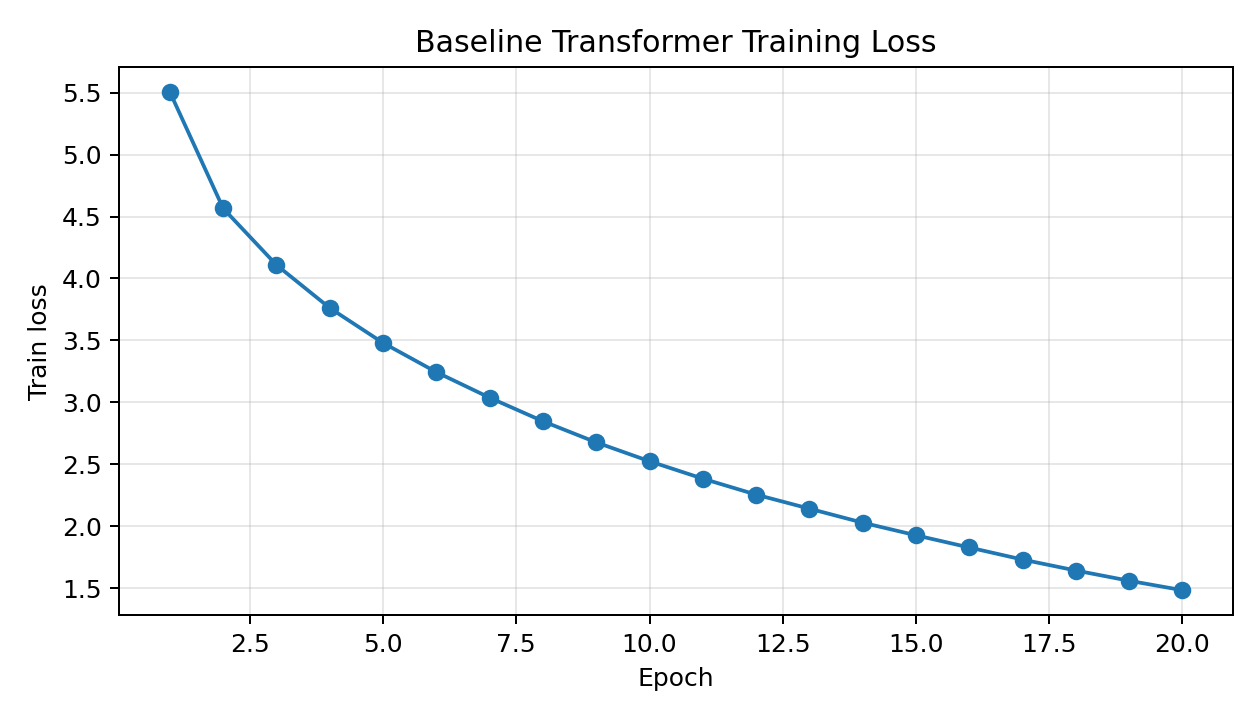
\includegraphics[width=0.72\textwidth]{../outputs/part1_machine_translation/baseline_default_6_layer/baseline_loss_curve.png}
\caption{Baseline Transformer 训练损失曲线}
\label{fig:baseline-loss}
\end{figure}

测试集 BLEU 由统一中文分词 BLEU 口径计算：先用 \texttt{jieba} 对参考译文和模型输出分词，再计算 corpus BLEU。按该口径，default 6-layer baseline 的 test BLEU 为 0.1579。训练脚本只负责在验证集上选择 checkpoint，并生成测试集预测文件；最终测试集分数统一由相同 BLEU 流程给出，避免不同实验之间出现评分口径不一致的问题。

表 \ref{tab:baseline-examples} 展示了测试集中的若干翻译样例。

\begin{table}[H]
\centering
\caption{Baseline 测试集翻译样例}
\label{tab:baseline-examples}
\begin{tabular}{p{0.24\textwidth}p{0.24\textwidth}p{0.24\textwidth}p{0.18\textwidth}}
\toprule
英文输入 & 参考译文 & 模型输出 & 分析 \\
\midrule
UNK ! & 干杯! & 转！ & 未登录英文词被映射为 \texttt{UNK}，模型难以恢复具体语义。 \\
listen . & 听着。 & 听听。 & 捕捉到动词大意，但短句中仍存在重复生成。 \\
try it . & 试试吧。 & 试试试。 & 语义接近，但输出重复，缺少语气词。 \\
no way ! & 不可能！ & 不要！ & 学到否定语气，但没有准确表达 ``不可能''。 \\
drive safely . & 安全地驾驶。 & 安静。 & 将 ``safely'' 与相近中文词混淆，遗漏驾驶动作。 \\
\bottomrule
\end{tabular}
\end{table}

从样例可以看到，default 6-layer baseline 已经能学习到部分短句的核心语义，例如 ``listen'' 和 ``try it'' 的输出与参考译文有明显重合；但模型仍存在三个明显问题：第一，遇到 \texttt{UNK} 或低频表达时容易生成无关词；第二，短句中仍有重复生成现象；第三，某些词义相近但语义不同的中文词会被混淆，例如 ``drive safely'' 被译为 ``安静''。这些问题说明 baseline 已具备基本翻译能力，但仍需要通过学习率调度改善收敛和生成质量。

\subsection{1.3 Cosine Warm-up 学习率策略}

本小节在 1.2 baseline 训练流程上新增 warm-up 与 cosine decay 组合的学习率调度，主要新增文件为 \path|code/part1_machine_translation/translator_en2cn_cosine.py|。除学习率调度外，数据划分、模型结构、batch size、训练轮数、验证间隔、checkpoint 保存间隔均与 baseline 保持一致。实验固定 warm-up 为 5 个 epoch，只改变 peak learning rate，从而观察峰值学习率对 loss 和 BLEU 的影响。示例训练命令如下：
\begin{lstlisting}[language=bash]
python code/part1_machine_translation/translator_en2cn_cosine.py \
  --name cosine_default_6_layer_peak3e-4 \
  --peak-lr 0.0003 \
  --warmup-epochs 5 \
  --min-lr 0.000001 \
  --epochs 20 \
  --batch-size 64 \
  --n-layer 6 \
  --heads 8 \
  --d-model 256 \
  --d-ff 1024 \
  --eval-every 5 \
  --save-every 5
\end{lstlisting}

设当前 epoch 为 $e$，总 epoch 数为 $T$，warm-up epoch 数为 $T_{warmup}$，峰值学习率为 $\eta_{peak}$，最小学习率为 $\eta_{min}$。本实验采用的学习率为：
\[
\eta(e)=
\begin{cases}
\eta_{peak}\frac{e}{T_{warmup}}, & e \leq T_{warmup} \\
\eta_{min}+\frac{1}{2}(\eta_{peak}-\eta_{min})
\left(1+\cos\left(\pi\frac{e-T_{warmup}}{T-T_{warmup}}\right)\right), & e > T_{warmup}
\end{cases}
\]

Warm-up 的作用是在训练初期把学习率从较小值逐步提升到峰值，避免模型参数随机初始化时受到过大更新而不稳定；cosine decay 的作用是在训练后期逐渐降低学习率，使参数更新更细致，帮助模型在较优区域附近收敛。每组实验均保存 \texttt{best\_model.pt}、\texttt{checkpoint\_epoch\_*.pt}、\texttt{config.json}、\texttt{loss\_history.json}、\texttt{metrics\_history.json}、\texttt{test\_predictions.txt} 和 \texttt{loss\_curve.png}。测试集 BLEU 使用与 1.2 相同的中文分词 BLEU 口径计算。

\begin{table}[H]
\centering
\caption{Cosine warm-up 不同峰值学习率实验结果}
\label{tab:cosine}
\resizebox{\textwidth}{!}{%
\begin{tabular}{lrrrrrl}
\toprule
实验名 & warmup epoch & peak lr & min lr & final train loss & valid BLEU & test BLEU \\
\midrule
Baseline fixed lr & -- & $1\times10^{-4}$ & -- & 1.4847 & 0.1698 & 0.1579 \\
Cosine A & 5 & $1\times10^{-4}$ & $1\times10^{-6}$ & 2.3193 & 0.1014 & 0.0947 \\
Cosine B & 5 & $2\times10^{-4}$ & $1\times10^{-6}$ & 1.3627 & 0.1824 & 0.1708 \\
Cosine C & 5 & $3\times10^{-4}$ & $1\times10^{-6}$ & 0.8725 & 0.2171 & 0.1999 \\
Cosine D & 5 & $4\times10^{-4}$ & $1\times10^{-6}$ & 0.5912 & 0.2344 & 0.2193 \\
Cosine E & 5 & $5\times10^{-4}$ & $1\times10^{-6}$ & 0.4302 & 0.2445 & 0.2270 \\
Cosine F & 5 & $6\times10^{-4}$ & $1\times10^{-6}$ & 0.3315 & 0.2460 & 0.2293 \\
Cosine G & 5 & $7\times10^{-4}$ & $1\times10^{-6}$ & 0.2735 & 0.2486 & 0.2339 \\
Cosine H & 5 & $8\times10^{-4}$ & $1\times10^{-6}$ & 0.2341 & 0.2550 & 0.2309 \\
\bottomrule
\end{tabular}
}
\end{table}

从表 \ref{tab:cosine} 可以看到，Cosine A 的 peak lr 与 baseline 的固定学习率相同，但由于 warm-up 前期学习率较低，且 cosine decay 后期持续下降到 $1\times10^{-6}$，整体训练更新偏保守，最终 train loss 和 BLEU 均低于 baseline。将 peak lr 提高到 $2\times10^{-4}$ 后，final train loss 降至 1.3627，valid BLEU 和 test BLEU 均超过 baseline，说明更高的峰值学习率弥补了 warm-up 和 decay 带来的平均学习率下降。

继续增大 peak lr 后，valid BLEU 从 $3\times10^{-4}$ 到 $8\times10^{-4}$ 基本持续上升，其中 Cosine H 即 \texttt{peak\_lr=8e-4,warmup=5} 取得最高 validation BLEU 0.2550。若观察 test BLEU，Cosine G 即 \texttt{peak\_lr=7e-4,warmup=5} 最高，达到 0.2339；Cosine H 的 test BLEU 为 0.2309，略低于 Cosine G。这说明在 $7\times10^{-4}$ 到 $8\times10^{-4}$ 附近模型性能已经接近平台期，继续增大学习率虽然可能进一步降低训练 loss，但未必稳定提升测试集泛化效果。

相比 fixed-lr baseline 的 test BLEU 0.1579，已测试学习率范围内的最佳 test BLEU 提升到 0.2339，提升约 0.0760。该结果说明，在 default 结构配置和 20 个 epoch 的训练预算下，warm-up cosine 调度配合合适的 peak learning rate 可以显著改善收敛速度和翻译质量；同时，过低的 peak learning rate 会导致更新不足，而过高的 peak learning rate 附近则可能出现 validation BLEU 与 test BLEU 不完全一致的现象。因此，本实验按照 validation BLEU 选择 \texttt{peak\_lr=8e-4} 作为调度配置，同时报告 \texttt{peak\_lr=7e-4} 在测试集上取得最高 BLEU。

\subsection{1.4 Transformer 结构消融实验}

本小节在 1.3 调参结果的基础上进行结构消融实验。由于 \texttt{peak\_lr=8e-4} 虽然取得最高 validation BLEU，但测试集 BLEU 略低于 \texttt{peak\_lr=7e-4}；而 \texttt{peak\_lr=7e-4} 在 test BLEU 上最高，泛化表现更稳定，因此本小节统一采用 \texttt{peak\_lr=7e-4,warmup=5,min\_lr=1e-6} 作为学习率策略。对照组直接复用 1.3 中的 \texttt{cosine\_default\_6\_layer\_peak7e-4}，其结构为 default 6-layer Transformer：\texttt{n\_layer=6,heads=8,d\_model=256,d\_ff=1024}。

消融实验只改变一个结构因素，其余训练设置保持一致，包括数据划分、batch size、epoch 数、warm-up cosine 调度、验证与 checkpoint 间隔，以及 BLEU 计算口径。具体比较了三种结构变化：减少 encoder/decoder 层数到 3 层、减少 attention head 数到 4 个、以及把 hidden size 从 256 降到 128 并相应将 \texttt{d\_ff} 从 1024 降到 512。

\begin{table}[H]
\centering
\caption{Transformer 结构消融实验结果（peak lr = $7\times10^{-4}$）}
\label{tab:ablation}
\resizebox{\textwidth}{!}{%
\begin{tabular}{lrrrrrrr}
\toprule
实验名 & n\_layer & heads & d\_model & d\_ff & final train loss & valid BLEU & test BLEU \\
\midrule
Default 6-layer 对照组 & 6 & 8 & 256 & 1024 & 0.2735 & 0.2486 & 0.2339 \\
Layer ablation & 3 & 8 & 256 & 1024 & 0.2800 & 0.2465 & 0.2259 \\
Head ablation & 6 & 4 & 256 & 1024 & 0.3064 & 0.2432 & 0.2351 \\
Hidden-size ablation & 6 & 8 & 128 & 512 & 1.0450 & 0.2055 & 0.1852 \\
\bottomrule
\end{tabular}
}
\end{table}

从表 \ref{tab:ablation} 可以看到，将层数从 6 层减少到 3 层后，final train loss 仅从 0.2735 上升到 0.2800，valid BLEU 也只从 0.2486 降到 0.2465，说明在当前数据规模和 20 个 epoch 训练预算下，3 层模型仍然具有较强的拟合能力。但 test BLEU 从 0.2339 降到 0.2259，下降约 0.0080，说明更浅的模型在泛化翻译质量上仍有损失，6 层结构能提供更充分的表示能力。

将 attention head 数从 8 减少到 4 后，train loss 上升到 0.3064，valid BLEU 降到 0.2432，说明多头注意力并行建模不同对齐关系的能力有所减弱。不过该组 test BLEU 为 0.2351，略高于对照组的 0.2339。这一差异很小，可能来自训练随机性、checkpoint 选择或测试集样本波动；结合 valid BLEU 和 loss，不能简单认为 4-head 结构整体优于 8-head，只能说明在本次测试集上 4-head 没有造成明显退化。

最明显的性能下降来自 hidden size 消融。当 \texttt{d\_model} 从 256 降到 128、\texttt{d\_ff} 从 1024 降到 512 后，final train loss 上升到 1.0450，valid BLEU 降到 0.2055，test BLEU 降到 0.1852。该结果说明模型宽度是当前翻译系统的重要容量来源；降低 hidden size 会同时削弱 embedding、attention 投影、feed-forward network 和最终 decoder 表示能力，使模型即使在训练集上也难以达到 default 配置的收敛水平。

综合来看，default 6-layer 配置仍是本组实验中最稳妥的结构选择。减少层数带来轻微但稳定的 test BLEU 下降，减少 head 数影响较小但验证集表现略差，而降低 hidden size 会显著损害收敛和 BLEU。因此，在后续使用机器翻译模型作为基础模型时，优先保留 \texttt{d\_model=256,d\_ff=1024} 的宽度配置，并使用 \texttt{n\_layer=6,heads=8} 的 default 结构。

\subsection{1.5 位置嵌入实验}

本小节比较不同位置嵌入方式对机器翻译性能的影响。Transformer 的 self-attention 本身不包含 token 顺序信息，因此需要额外加入 position encoding。前面 1.2--1.4 的模型均使用固定 sinusoidal position encoding；本小节新增 learnable positional embedding，并在 \texttt{build\_transformer} 中加入 \texttt{pe\_type} 参数，使模型可以在 \texttt{sinusoidal} 和 \texttt{learnable} 两种位置嵌入之间切换。

为了避免重复训练，本小节的 sinusoidal 对照组直接复用 1.3/1.4 中的 \texttt{cosine\_default\_6\_layer\_peak7e-4} 结果。该模型使用 default 6-layer 结构和固定 sinusoidal position encoding，且学习率策略为 \texttt{peak\_lr=7e-4}、\texttt{warmup=5}、\texttt{min\_lr=1e-6}。实验组 \texttt{pe\_learnable\_peak7e-4} 只将位置嵌入改为可学习参数，其余设置保持一致：\texttt{n\_layer=6}、\texttt{heads=8}、\texttt{d\_model=256}、\texttt{d\_ff=1024}，并使用相同 batch size、epoch 数、数据划分和 BLEU 计算口径。

\begin{table}[H]
\centering
\caption{位置嵌入方式实验结果}
\label{tab:position-embedding}
\resizebox{\textwidth}{!}{%
\begin{tabular}{llrrrr}
\toprule
实验名 & 位置嵌入类型 & final train loss & valid BLEU & test BLEU & best epoch \\
\midrule
\texttt{cosine\_default\_6\_layer\_peak7e-4} & sinusoidal & 0.2735 & 0.2486 & 0.2339 & 20 \\
\texttt{pe\_learnable\_peak7e-4} & learnable & 0.2559 & 0.2343 & 0.2229 & 20 \\
\bottomrule
\end{tabular}
}
\end{table}

从表 \ref{tab:position-embedding} 可以看到，learnable position embedding 的 final train loss 为 0.2559，低于 sinusoidal 对照组的 0.2735，说明可学习位置参数能够进一步适应训练集分布，使训练目标略有改善。但在 BLEU 指标上，learnable PE 的 valid BLEU 为 0.2343，低于 sinusoidal 的 0.2486；test BLEU 为 0.2229，也低于 sinusoidal 的 0.2339。这说明在当前数据规模和训练预算下，可学习位置嵌入虽然降低了训练 loss，但没有带来更好的验证集和测试集翻译质量。

造成这一现象的可能原因是，sinusoidal position encoding 提供了稳定的固定位置先验，不需要从有限训练数据中学习位置模式，因此在小规模平行语料上更容易泛化。Learnable PE 增加了额外参数，理论上可以学习更贴合任务的位置表示，但也更依赖数据规模和优化稳定性；当训练数据较少时，它可能更容易贴合训练集而不能稳定提升 BLEU。因此，本实验中仍选择 sinusoidal PE 作为更稳妥的位置嵌入方式，并沿用 \texttt{cosine\_default\_6\_layer\_peak7e-4} 作为第一部分后续 encoder checkpoint 的优先候选。

\subsection{第一部分小结}

本部分完成了 English-to-Chinese Transformer 翻译系统的实现、default 6-layer baseline 训练与 BLEU 评估，并在 1.3 中进一步比较了 warm-up cosine 学习率调度下不同 peak learning rate 的效果。从实验结果看，baseline Transformer 可以正常收敛并生成翻译结果；引入 cosine warm-up 后，\texttt{peak\_lr=8e-4,warmup=5} 取得最高 validation BLEU，\texttt{peak\_lr=7e-4,warmup=5} 取得最高 test BLEU。测试集 BLEU 从 fixed-lr baseline 的 0.1579 提升到最高 0.2339，说明在固定 default 模型结构和 20 个 epoch 训练轮数时，适当提高峰值学习率可以改善收敛速度和翻译质量，而过低的 peak learning rate 会因为 warm-up 与 cosine decay 的共同作用导致整体更新不足。1.4 的结构消融进一步显示，模型宽度对翻译性能影响最大，将 \texttt{d\_model} 降到 128 会明显损害收敛和 BLEU；减少层数会带来轻微泛化下降；减少 attention head 数影响较小但验证集表现略低。1.5 的位置嵌入实验显示，learnable PE 虽然取得更低训练 loss，但 validation/test BLEU 均低于 sinusoidal PE。综合 1.3--1.5，后续优先采用 \texttt{peak\_lr=7e-4,warmup=5}、default 6-layer 结构与 sinusoidal position encoding 作为更稳妥的机器翻译配置。
\section{第二部分：Tweet Sentiment 情感分析}

本部分使用第一部分训练得到的 English-to-Chinese Transformer encoder 作为预训练表示模块，在 Tweet Sentiment Extraction 数据集上进行情感分类微调。数据集来源为 Hugging Face 的 \texttt{mteb/tweet\_sentiment\_extraction}，本地使用下载后的 \texttt{train.jsonl} 和 \texttt{test.jsonl}。每条样本包含 tweet 文本和情感标签，标签包括 \texttt{negative}、\texttt{neutral} 和 \texttt{positive} 三类。

\subsection{2.1 基于翻译 Encoder 的情感分类微调}

本小节对应情感分析的 baseline 微调实验。按照题目要求，模型必须加载第一部分训练得到的 encoder 预训练参数，因此本实验选择第一部分综合表现最稳的 checkpoint：
\begin{lstlisting}
outputs/part1_machine_translation/cosine_default_6_layer_peak7e-4/best_model.pt
\end{lstlisting}
该 checkpoint 使用 default 6-layer Transformer 结构、sinusoidal position encoding 和 \texttt{peak\_lr=7e-4,warmup=5} 的学习率策略，在第一部分取得 test BLEU 0.2339。

模型结构上，原始翻译模型的 decoder 和 projection layer 被移除，只保留 source embedding、source position encoding 和 encoder。输入 tweet 按第一部分英文词表进行 tokenization，并加入 \texttt{BOS}/\texttt{EOS} 标记；未登录词映射到 \texttt{UNK}，padding 位置通过 attention mask 屏蔽。Encoder 输出为每个 token 的 hidden state，本实验默认使用 mean pooling 对所有非 padding token 的表示取平均，得到句子级向量，再通过一个线性分类头输出三类情感 logits。训练损失使用交叉熵：
\[
\mathcal{L}=-\sum_{c=1}^{C} y_c \log p_c
\]
其中 $C=3$，分别对应 \texttt{negative}、\texttt{neutral} 和 \texttt{positive}。

训练脚本为 \texttt{code/part2\_sentiment\_analysis/train\_sentiment.py}，模型定义为 \texttt{code/part2\_sentiment\_analysis/sentiment\_model.py}。实验从 \texttt{train.jsonl} 中按标签比例划分训练集和验证集，并使用官方 \texttt{test.jsonl} 作为测试集。具体数据规模如表 \ref{tab:sentiment-data} 所示。

\begin{table}[H]
\centering
\caption{Tweet Sentiment 数据划分}
\label{tab:sentiment-data}
\begin{tabular}{lr}
\toprule
划分 & 样本数 \\
\midrule
Train & 21984 \\
Validation & 2748 \\
Test & 2749 \\
\bottomrule
\end{tabular}
\end{table}

主要训练配置如表 \ref{tab:sentiment-config} 所示。由于本任务是微调任务，encoder 已经从机器翻译任务中获得初始化参数，因此学习率设置为 $2\times10^{-4}$，低于第一部分机器翻译中从零训练时使用的 peak learning rate，以减少对预训练表示的破坏。训练总轮数设为 8，并根据 validation accuracy 保存最佳模型。

\begin{table}[H]
\centering
\caption{情感分类微调配置}
\label{tab:sentiment-config}
\begin{tabular}{lr}
\toprule
配置项 & 取值 \\
\midrule
预训练 checkpoint & \texttt{cosine\_default\_6\_layer\_peak7e-4} \\
Encoder 层数 & 6 \\
Hidden size & 256 \\
Attention heads & 8 \\
Pooling & mean pooling \\
Batch size & 64 \\
Epochs & 8 \\
Learning rate & $2\times10^{-4}$ \\
Weight decay & 0.01 \\
Loss & CrossEntropyLoss \\
\bottomrule
\end{tabular}
\end{table}

\begin{figure}[H]
\centering

\includegraphics[width=0.72\textwidth]{../outputs/part2_sentiment_analysis/sentiment_baseline/loss_curve.png}
\caption{情感分类训练与验证 loss 曲线}
\label{fig:sentiment-loss}
\end{figure}

\begin{figure}[H]
\centering
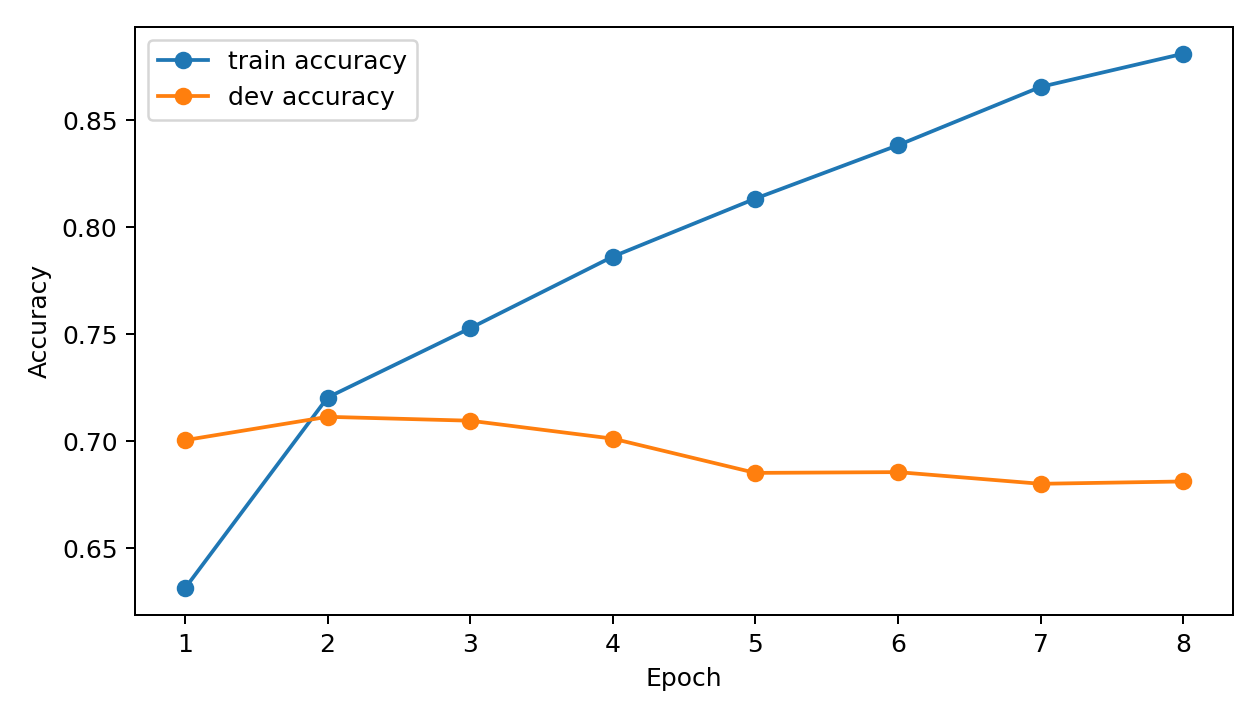
\includegraphics[width=0.72\textwidth]{../outputs/part2_sentiment_analysis/sentiment_baseline/accuracy_curve.png}
\caption{情感分类训练与验证 accuracy 曲线}
\label{fig:sentiment-acc}
\end{figure}

从图 \ref{fig:sentiment-loss} 和图 \ref{fig:sentiment-acc} 可以看到，训练集 loss 从第 1 轮的 0.8190 持续下降到第 8 轮的 0.3095，训练 accuracy 从 0.6313 上升到 0.8810，说明模型能够有效拟合情感分类训练集。验证集 accuracy 在第 2 轮达到最高 0.7114，此后虽然训练集继续改善，但验证 loss 从 0.7082 上升到 1.0888，验证 accuracy 也逐步下降到 0.6812。这说明模型在第 2 轮之后开始明显过拟合，因此最终测试使用 validation accuracy 最优的第 2 轮 checkpoint。

\begin{table}[H]
\centering
\caption{情感分类训练过程记录}
\label{tab:sentiment-history}
\begin{tabular}{rrrrr}
\toprule
Epoch & train loss & train acc & valid loss & valid acc \\
\midrule
1 & 0.8190 & 0.6313 & 0.7190 & 0.7005 \\
2 & 0.6627 & 0.7204 & 0.7082 & 0.7114 \\
3 & 0.5962 & 0.7528 & 0.7228 & 0.7096 \\
4 & 0.5346 & 0.7863 & 0.7503 & 0.7012 \\
5 & 0.4734 & 0.8134 & 0.8218 & 0.6852 \\
6 & 0.4121 & 0.8383 & 0.8797 & 0.6856 \\
7 & 0.3535 & 0.8655 & 0.9535 & 0.6801 \\
8 & 0.3095 & 0.8810 & 1.0888 & 0.6812 \\
\bottomrule
\end{tabular}
\end{table}

最终测试集结果如表 \ref{tab:sentiment-class-test} 和表 \ref{tab:sentiment-overall-test} 所示。模型在测试集上取得 accuracy 0.7097，macro F1 为 0.7137，weighted F1 为 0.7095。分类别来看，\texttt{positive} 的 F1 最高，达到 0.7699；\texttt{negative} 的 F1 为 0.7054；\texttt{neutral} 的 F1 相对较低，为 0.6657。这与 tweet 情感分类任务的特点一致：中性类别边界更模糊，容易与轻微正向或负向表达混淆。

\begin{table}[H]
\centering
\caption{情感分类测试集分类别结果}
\label{tab:sentiment-class-test}
\begin{tabular}{lrrrr}
\toprule
类别 & Precision & Recall & F1 & Support \\
\midrule
negative & 0.6725 & 0.7416 & 0.7054 & 778 \\
neutral & 0.6851 & 0.6475 & 0.6657 & 1112 \\
positive & 0.7786 & 0.7614 & 0.7699 & 859 \\
\bottomrule
\end{tabular}
\end{table}

\begin{table}[H]
\centering
\caption{情感分类测试集总体结果}
\label{tab:sentiment-overall-test}
\begin{tabular}{lr}
\toprule
指标 & 数值 \\
\midrule
Accuracy & 0.7097 \\
Macro Precision & 0.7120 \\
Macro Recall & 0.7168 \\
Macro F1 & 0.7137 \\
Weighted Precision & 0.7107 \\
Weighted Recall & 0.7097 \\
Weighted F1 & 0.7095 \\
Test samples & 2749 \\
\bottomrule
\end{tabular}
\end{table}

总体而言，加载机器翻译 encoder 后，模型能够在较少 epoch 内达到约 71\% 的测试准确率，说明第一部分 encoder 学到的英文 token 表示对情感分类有一定迁移价值。但训练后期出现过拟合，也说明 tweet sentiment 数据与机器翻译任务存在明显差异，后续需要通过 early stopping、冻结部分 encoder、调整学习率或比较有无位置嵌入等实验进一步分析模型泛化能力。

\subsection{2.2 Position Encoding 对情感分类的影响}

第一部分 1.5 已经比较了 sinusoidal position encoding 和 learnable position embedding 在机器翻译任务中的差异。本小节进一步分析位置嵌入对 Tweet Sentiment 情感分类迁移任务的影响。对照组直接复用 2.1 的 \texttt{sentiment\_baseline}，即保留从机器翻译 checkpoint 加载的 source embedding、source position encoding 和 encoder；实验组 \texttt{sentiment\_without\_pe} 在相同 checkpoint 初始化、相同数据划分和相同训练配置下关闭 position embedding，只使用 token embedding 经过 encoder 后进行 mean pooling 和三分类。

两组实验均使用相同训练配置：训练 8 个 epoch，batch size 为 64，学习率为 $2\times10^{-4}$，weight decay 为 0.01，并采用 mean pooling。主要结果如表 \ref{tab:sentiment-pe-overall} 所示。

\begin{table}[H]
\centering
\caption{有无 position encoding 的情感分类总体结果}
\label{tab:sentiment-pe-overall}
\begin{tabular}{lrrrrr}
\toprule
设置 & Best epoch & Dev acc & Test loss & Test acc & Macro F1 \\
\midrule
with PE & 2 & 0.7114 & 0.6854 & 0.7097 & 0.7137 \\
without PE & 3 & 0.7060 & 0.7058 & 0.7148 & 0.7167 \\
\bottomrule
\end{tabular}
\end{table}

从总体指标看，关闭 position encoding 后，最佳 validation accuracy 从 0.7114 略降到 0.7060，说明带有位置信息的 encoder 在验证集上仍有轻微优势；但在测试集上，without PE 的 accuracy 从 0.7097 提升到 0.7148，macro F1 从 0.7137 提升到 0.7167。两者差距都很小，因此不能说明关闭 position encoding 带来了稳定显著的提升，更合理的结论是：在当前 tweet sentiment 分类任务中，位置嵌入不是决定性能的关键因素。

分类别结果如表 \ref{tab:sentiment-pe-class} 所示。Without PE 对 \texttt{neutral} 类别的 F1 从 0.6657 提升到 0.6933，但 \texttt{negative} 和 \texttt{positive} 的 F1 略低于 with PE。由于 \texttt{neutral} 类别本身边界更模糊，这一变化使 without PE 的 macro F1 略高，但不同类别之间的增减并不完全一致。

\begin{table}[H]
\centering
\caption{有无 position encoding 的情感分类分类别 F1 对比}
\label{tab:sentiment-pe-class}
\begin{tabular}{lrr}
\toprule
类别 & with PE F1 & without PE F1 \\
\midrule
negative & 0.7054 & 0.6964 \\
neutral & 0.6657 & 0.6933 \\
positive & 0.7699 & 0.7605 \\
\bottomrule
\end{tabular}
\end{table}

这一结果与第一部分 1.5 的机器翻译实验形成对比。在 English-to-Chinese translation 中，模型需要处理源句和目标句之间的顺序、句法结构和跨语言对齐关系，position encoding 直接影响 attention 对 token 顺序的建模能力，因此 sinusoidal PE 在 validation/test BLEU 上明显优于 learnable PE，并且位置建模对翻译质量较为关键。相比之下，Tweet Sentiment 更依赖情感词、短语和局部语义线索，例如正负向形容词、否定表达、语气词等；句子整体类别通常可以通过词汇线索和短文本语义聚合判断，mean pooling 也进一步弱化了精确位置顺序的作用。因此，即使关闭 position encoding，模型仍能取得与 baseline 接近的测试表现。

综合 2.1 和 2.2，可以认为第一部分迁移来的 encoder 对情感分类有效，但 position encoding 在该分类任务中的收益有限。后续若继续改进情感分类，更值得优先尝试 early stopping、冻结部分 encoder、降低学习率或加入更强的正则化，而不是单独依赖位置嵌入设置。

\section{第三部分：Vision Transformer 与 ResNet 对比}

本部分在 CIFAR-10 图像分类任务上实现 Vision Transformer，并与 ResNet50 卷积网络进行对比。数据读取流程参考 PyTorch 官方 CIFAR-10 分类教程，使用 torchvision 的 CIFAR-10 数据集接口构建训练集和测试集。原始 50000 张训练图像按照类别分层划分为 45000 张训练样本和 5000 张验证样本，官方 10000 张测试图像作为最终测试集。训练图像使用 random crop 和 horizontal flip 进行数据增强，验证集和测试集只进行 tensor 转换和 normalization。

\subsection{3.1 Vision Transformer on CIFAR-10}

ViT 代码位于 \path|code/part3_vision_transformer/vit_model.py| 和 \path|code/part3_vision_transformer/train_vit.py|。模型首先将 $32\times32$ RGB 图像划分为 $4\times4$ patch，因此每张图像得到 $8\times8=64$ 个 patch。Patch embedding 使用一个 kernel size 和 stride 均为 4 的卷积实现，等价于把每个 patch flatten 后映射到 hidden dimension。随后在 patch 序列前加入 learnable class token，并叠加 learnable position embedding。序列输入 Transformer encoder，最终使用 class token 的输出经过线性分类头得到 10 类 CIFAR-10 logits。

本实验使用较小的 ViT 配置以适应 CIFAR-10 和当前训练预算：\texttt{embed\_dim=192}、\texttt{depth=6}、\texttt{num\_heads=6}、\texttt{mlp\_dim=384}、\texttt{patch\_size=4}，参数量约 1.81M。优化器为 AdamW，学习率 $3\times10^{-4}$，weight decay 为 0.05，使用 cosine annealing 调度，训练 20 个 epoch。主要配置和结果如表 \ref{tab:vit-config-result} 所示。

\begin{table}[H]
\centering
\caption{ViT CIFAR-10 训练配置与结果}
\label{tab:vit-config-result}
\begin{tabular}{lr}
\toprule
项目 & 数值 \\
\midrule
Patch size & 4 \\
Patch 数量 & 64 \\
Hidden size & 192 \\
Transformer layers & 6 \\
Attention heads & 6 \\
MLP hidden size & 384 \\
Train / Validation / Test & 45000 / 5000 / 10000 \\
Epochs & 20 \\
Best epoch & 19 \\
Best validation accuracy & 0.7364 \\
Test accuracy & 0.7276 \\
Test loss & 0.7711 \\
参数量 & 1.81M \\
训练时间 & 777.8 s \\
\bottomrule
\end{tabular}
\end{table}

\begin{figure}[H]
\centering

\includegraphics[width=0.72\textwidth]{../outputs/part3_vision_transformer/vit_cifar10/loss_curve.png}
\caption{ViT 在 CIFAR-10 上的 loss 曲线}
\label{fig:vit-loss}
\end{figure}

\begin{figure}[H]
\centering

\includegraphics[width=0.72\textwidth]{../outputs/part3_vision_transformer/vit_cifar10/accuracy_curve.png}
\caption{ViT 在 CIFAR-10 上的 accuracy 曲线}
\label{fig:vit-acc}
\end{figure}

从图 \ref{fig:vit-loss} 和图 \ref{fig:vit-acc} 可以看到，ViT 的训练 loss 从 1.7945 下降到 0.7349，训练 accuracy 从 0.3303 上升到 0.7384；验证 accuracy 从第 1 轮的 0.3894 逐步提升到第 19 轮的最高 0.7364，说明模型能够稳定学习 CIFAR-10 的视觉特征。最终测试 accuracy 为 0.7276，与验证集表现接近，没有出现明显的验证--测试分布偏差。

\subsection{3.2 ResNet50/CNN 对比}

为了满足题目中使用预训练 CNN 模型的要求，本小节使用 ImageNet 预训练的 ResNet50 作为 CNN 对比模型，训练脚本为 \path|code/part3_vision_transformer/train_resnet.py|。模型加载方式与题目参考代码一致，即调用 \texttt{torch.hub.load("pytorch/vision:v0.10.0","resnet50",pretrained=True)} 获得预训练 ResNet50。随后将原始 1000 类分类头替换为 10 类线性层，用于 CIFAR-10 分类。

由于该 ResNet50 在 ImageNet 的 $224\times224$ 图像上预训练，本实验将 CIFAR-10 图像 resize 到 $224\times224$，并使用 ImageNet mean/std 进行 normalization。训练时冻结 ResNet50 backbone，只训练新加入的 10 类分类头；这样既保留预训练视觉特征，也避免在 CIFAR-10 小数据集上对大规模 backbone 进行过度更新。ResNet50 使用与 ViT 相同的 train/validation/test 划分，训练 10 个 epoch，优化器为 AdamW，初始学习率 $1\times10^{-3}$，weight decay 为 0.01。结果如表 \ref{tab:vit-resnet-compare} 所示。

\begin{table}[H]
\centering
\caption{ViT 与预训练 ResNet50 在 CIFAR-10 上的结果对比}
\label{tab:vit-resnet-compare}
\begin{tabular}{lrrrrr}
\toprule
模型 & Epochs & 可训练参数 & Best val acc & Test acc & 训练时间(s) \\
\midrule
ViT & 20 & 1.81M & 0.7364 & 0.7276 & 777.8 \\
Pretrained ResNet50 & 10 & 0.02M & 0.8286 & 0.8212 & 1560.0 \\
\bottomrule
\end{tabular}
\end{table}

\begin{figure}[H]
\centering

\includegraphics[width=0.72\textwidth]{../outputs/part3_vision_transformer/resnet50_cifar10/loss_curve.png}
\caption{预训练 ResNet50 在 CIFAR-10 上的 loss 曲线}
\label{fig:resnet-loss}
\end{figure}

\begin{figure}[H]
\centering

\includegraphics[width=0.72\textwidth]{../outputs/part3_vision_transformer/resnet50_cifar10/accuracy_curve.png}
\caption{预训练 ResNet50 在 CIFAR-10 上的 accuracy 曲线}
\label{fig:resnet-acc}
\end{figure}

预训练 ResNet50 的训练 loss 从 0.8815 下降到 0.4706，验证 accuracy 从 0.7850 提升到最高 0.8286，最终测试 accuracy 为 0.8212，高于从零训练 ViT 的 0.7276。该结果说明，ImageNet 预训练 CNN 已经学习到较通用的边缘、纹理和局部形状特征，即使只训练最后的分类头，也能较好迁移到 CIFAR-10。相比之下，ViT 从零训练时缺少卷积网络的局部结构先验，也没有大规模视觉预训练支持，因此在当前数据规模和训练预算下表现较弱。需要注意的是，本对比并不是完全等条件的结构公平比较：ResNet50 使用了 ImageNet 预训练知识，而 ViT 是从零训练；因此该实验更主要说明预训练 CNN 在小型图像分类任务上的迁移优势。

\section{总结}

本文完成了三个部分的实验。第一部分实现并训练 English-to-Chinese Transformer，通过学习率调度、结构消融和位置嵌入实验分析了机器翻译模型的关键因素；第二部分复用第一部分 encoder 进行 Tweet Sentiment 情感分类，验证了翻译 encoder 的迁移价值，并比较了 position encoding 对分类任务的影响；第三部分实现 ViT 并与 ImageNet 预训练 ResNet50 在 CIFAR-10 上对比，结果显示预训练 CNN 在小图像分类任务上具有明显迁移优势。整体来看，Transformer 在序列建模和跨任务迁移中表现灵活，但不同任务对顺序信息、局部结构、预训练和数据规模的依赖不同，需要结合任务特点选择模型结构和训练策略。

\end{document}


